\documentclass[conference]{IEEEtran}
%\IEEEoverridecommandlockouts
% The preceding line is only needed to identify funding in the first footnote. If that is unneeded, 
% please comment it out.
\usepackage{cite}
\usepackage{amsmath,amssymb,amsfonts}
\usepackage{algorithmic}
\usepackage{graphicx}
\usepackage{textcomp}
\usepackage{xcolor}
\def\BibTeX{{\rm B\kern-.05em{\sc i\kern-.025em b}\kern-.08em
    T\kern-.1667em\lower.7ex\hbox{E}\kern-.125emX}}
\begin{document}

\title{Development of a Data Lake System}

\author{\IEEEauthorblockN{A. Martin}
\IEEEauthorblockA{
\textit{Hochschule Niederrhein}\\
Krefeld, Germany \\
alexander.martin@stud.hn.de}
\and
\IEEEauthorblockN{M. Thiel}
\IEEEauthorblockA{
\textit{Hochschule Niederrhein}\\
Krefeld, Germany \\
marcel.thiel@stud.hn.de}
\and
\IEEEauthorblockN{R. Kuller}
\IEEEauthorblockA{
\textit{Hochschule Niederrhein}\\
Krefeld, Germany\\
robin.kuller@stud.hn.de}
}

\maketitle

% Version: 0.6

\begin{abstract}
% What is the project about?
The goal of this master project was to build a prototype data lake system based on a four-layered 
architecture, including an ingestion, a storage, a transformation and an interaction layer.
% How did we proceeded?
The data lake was built with \textit{Apache Spark} as the essential data-processing framework. In 
addition, several other frameworks and software were used, named later in section~\ref{ARC}.
% What are the most important results?
The final result of the project are simple APIs and  a UI, of which the most important feature is
the support and interoperability with different source- and target-systems. 
% What does the results imply?
This makes the project result a solid basis for extending and adjusting to the needs of different 
applications.
\end{abstract}

%--------------------------------------------------------------------------------------------------
\section{Introduction}\label{INT}
\subsection{Background}\label{BGD}
Nowadays many companies have a large number of (different) database systems, which store large 
quantities of data. 
A common difficulty is, to get a comprehensive overview of all the data.
In the worst case scenario, many so-called ``data silos'' exist. 
Having data silos mean that the data on each database system may be accessed, but to
get a connection between data from different systems is very difficult.
To get this connections and an overview of the data, some kind of data integration is needed.
A classical solution for data integration is a data warehouse system.
The main problem of these systems when dealing with big data, is the heterogeneity of data, 
because they use so called ``ETL'' processes. 
Since data get transformed into a uniform global scheme before they get stored, it is nearly 
impossible to ensure that this scheme is useful after merging many different types of data.

As a result, data lakes\cite{Quix2018} are a proposed solution\cite{Dixon2010} to deal with this 
problem.
The first step here is the ``\textbf{E}xtraction" and storing of data as-is.
Before the data can be processed, they have to be ``\textbf{L}oaded", so they are available.
The ``\textbf{T}ransformation" takes place as the last step right before one can work on the data. 
This concept is called ``\textbf{ELT}" and is the standout difference compared to a data warehouse 
system or other similar solutions. 
In this way the global scheme is bypassed, while the combination of different data is still possible
at a later stage, the transformation layer.

In recent years, many different systems (e.g. \textit{Apache Spark} or \textit{Apache Hadoop}, later 
referred to as \textit{Spark} and \textit{Hadoop}, respectively), which can be used to build a data
lake system, were implemented.
However, there is no well known open-source data lake solution available at the moment.


\subsection{Objectives}\label{AOB}
The main objective of this project was, to develop a prototype data lake system, based on the 
architecture explained in detail in section~\ref{USA}.
For the implementation no further spectifications were given.
The derived objectives for implementing the prototype were to decide on an architecure and to 
link several systems from different areas.

As a part of the transformation layer, \textit{Apache Nifi} (reffered to as \textit{Nifi}) was 
considered for creating (graphical) transformation workflows.
Therefore, \textit{Nifi} got analyzed, to define whether it is a valid option for this purpose.


%--------------------------------------------------------------------------------------------------
\section{Underlying Architecture}\label{USA}
To understand later explained design decisions on the architecture, the underlying data lake 
architecture in Fig.~\ref{DLA} will be described in this subsection.

Beneth the ingestion layer, different sources of heterogeneous data can be seen.
Those can be files, different kinds of database systems (e.g. relational, document-oriented, 
wide-column, graph-oriented etc.), other sources like clouds or simply a local computer.

At the bottom of the data lake architecture the \textbf{ingestion layer} is shown.
All different types of data shall be stored in their original form, but a certain data quality shall
be reached (e.g. usage of the same date format). 
During this ingestion, metadata shall be extracted automatically out of the given information.

In the \textbf{storage layer} besides the main data, referring metadata is stored. 
Because data are saved in its original form, multiple different storage systems are needed. 
However an uniform access point is needed, so data can be loaded by the system from any 
storage system.
Details about the content of the stored data are provided by metadata and data quality information.

Above, one can find the \textbf{transformation layer}.
In this layer stored data can be loaded and transformed, which means e.g. sorted or merged with 
other data (data integration).
A certain kind of data cleaning or preprocessing can take place before the transformation in some 
use cases, but this is not a necessary step. 
After editing some data, the results can be stored in a newly created application specific data 
mart, which can be utilized again from then on.

At the top of Fig.~\ref{DLA} the \textbf{interaction layer} can be spotted.
One can interact with the whole system in this layer.
Explorative as well as specified searches can be submitted over the whole data stored in the data 
lake system. 
As a result one can see, where the data of interest is stored, so one can decide afterwards on which 
data the transformations should be executed.
Another feature of this layer shall be an visualization of the data one is working on.

\begin{figure}[h]
\centerline{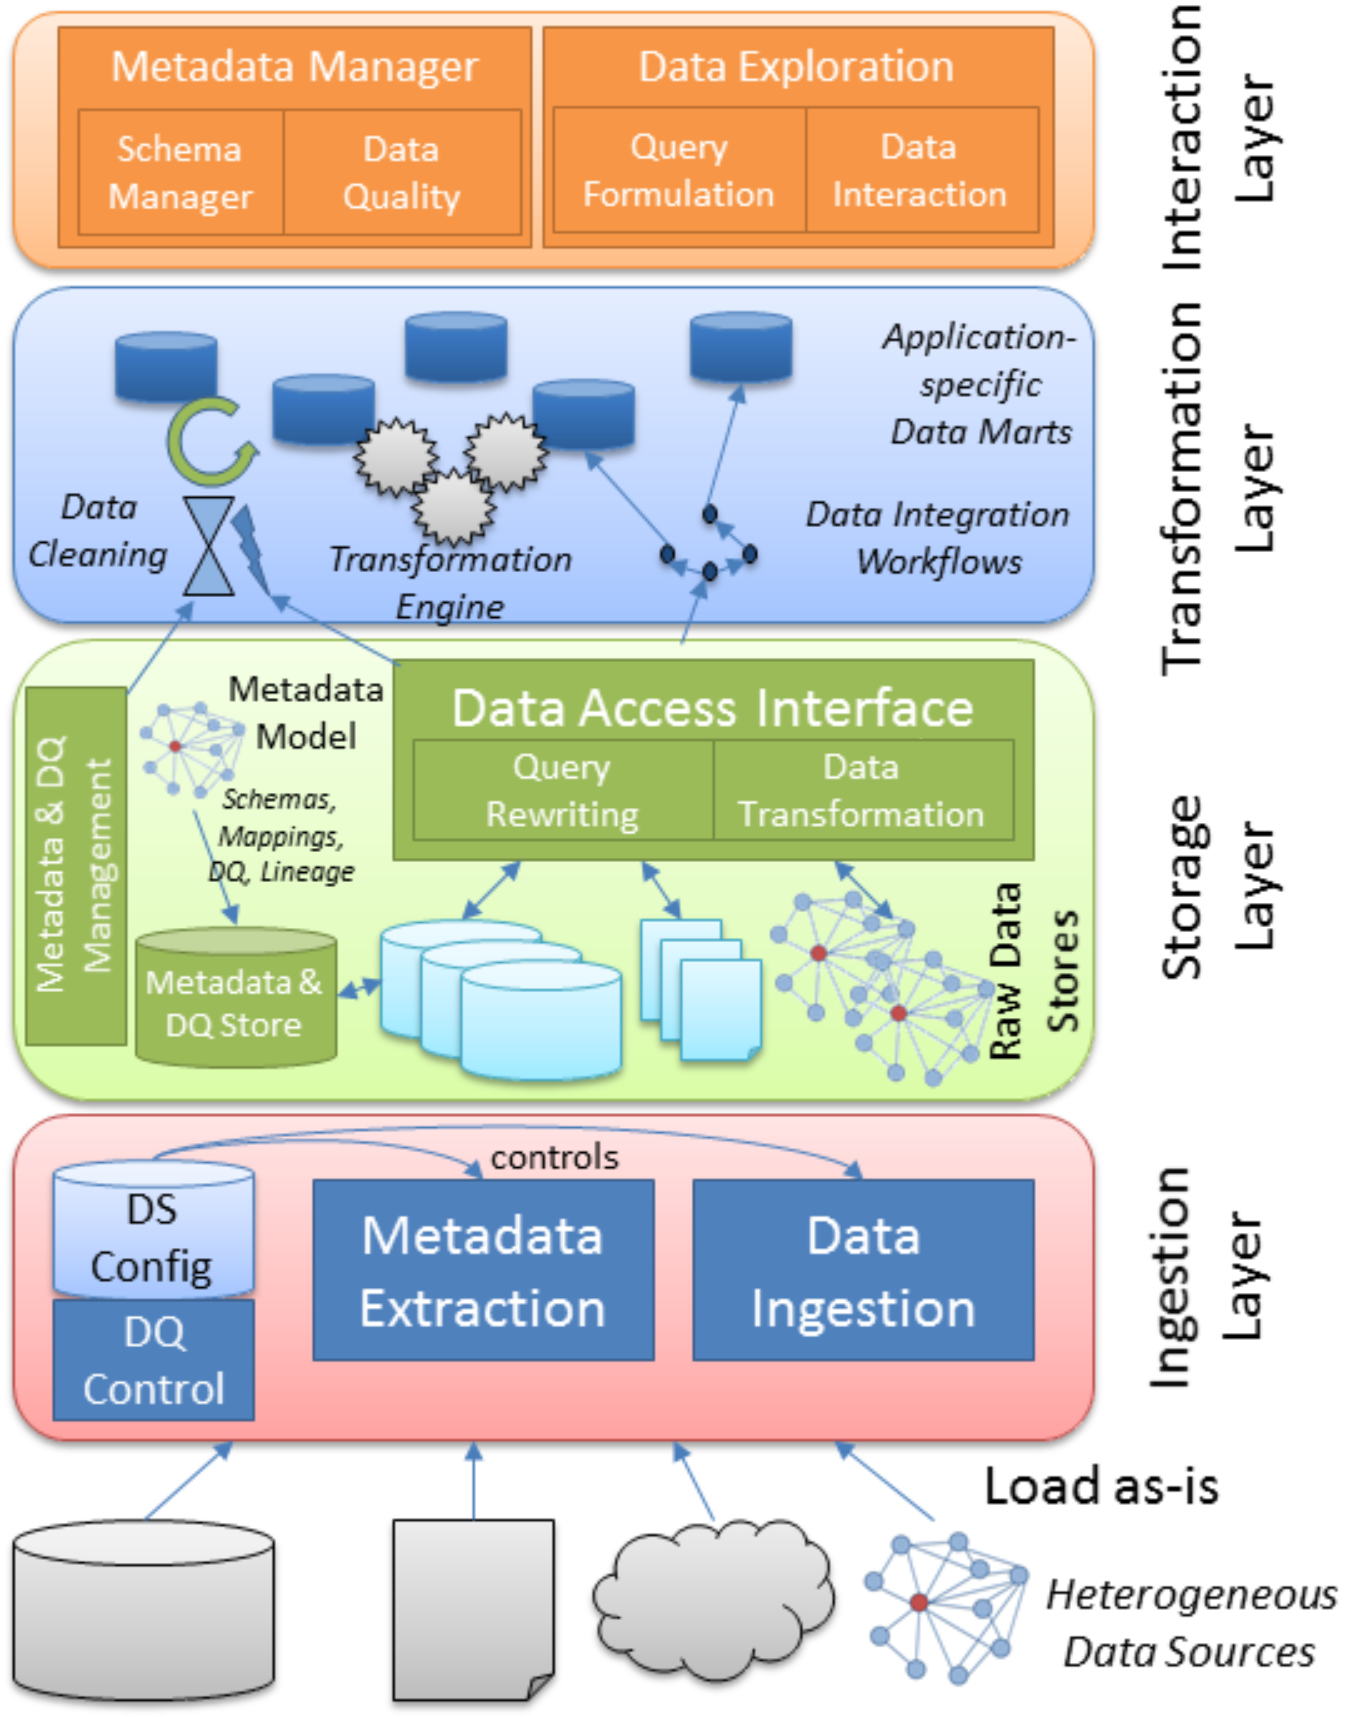
\includegraphics[scale=0.5]{graphics/data_lake_architecture.PNG}}
\caption{Underlying Data Lake Architecture\cite{Quix_Architecture}}
\label{DLA}
\end{figure}

%--------------------------------------------------------------------------------------------------
\section{Architecture}\label{ARC}
In this section our predecisions and our final architecture design will be introduced.
\subsection{Predecisions}\label{PRE}
To get a solution, which is independent from any use case we decided on a server-client 
architecture, with a REST API (Representational State Transfer Application Programming Interface) 
for communication. 
The realization of the client should only be an example of using the REST API.
The server should be usable for any purpose by any client.

As mentioned in subsection~\ref{AOB} \textit{Nifi} was analyzed for its possible usage in the 
transformation layer. 
\textit{Nifi} is a tool to automate data flow between (heterogeneous) systems. 
To work as intended, one can control and manage the processes in real-time between all source
and target systems.
A disadvantage of \textit{Nifi} is that it works with the ETL concept, which makes it less suitable
to function in a data lake system in general.
Furthermore, the tool has mainly vertical scalability, which does not fit well with the horizontal
scalability a data lake system naturally has.
Because of these disadvantages, we decided not to use \textit{Nifi} for this project.
Instead we will use solely \textit{Spark} in the transformation layer.

\subsection{Architecture Design}\label{ADN}
To describe the final architecture design of this project, Fig.~\ref{DLPA} shows a high-level 
overview of the structure of the data lake system.

As the data framework, \textit{Spark} was given. 
It is mainly used in the data lake for transformations in the corresponding layer. 
How it is used exactly, will be described in subsection~\ref{TFL}.
Secondly it is used in the ingestion layer to write DataFrames to the chosen target system.
These DataFrames are distributed collections of data organized into named columns in \textit{Spark}.

Because we choose to use a REST API for communication, a suitable solution for the backend was 
sought.
Different frameworks were examined (e.g. \textit{Apache Livy}), but in many cases the documentation
was insufficient.
In the end we decided to implement our own REST API using \textit{Flask}, which main advantages are 
scalability and a detailed documentation. 

At the bottom of Fig.~\ref{DLPA} the storage systems can be seen.
In the project we decided to use \textit{PostgreSQL} and \textit{MongoDB} as they are known examples of relational 
databases, respectively document-oriented NoSQL database systems.
Also we used \textit{HDFS} in a \textit{Hadoop}-cluster as a distributed storage system, as
it is commonly used in the field of big data.
The backend and \textit{Spark} are accessing the different storage systems.
As a part of the the backend the ``Data Access'' is used to manage the metadata stored in 
\textit{MongoDB}, but is also responsible for initializing the storage systems.
In section~\ref{RES} these processes are described more detailed.

We chose to implement the frontend as an own developed web client, because it is 
platform-independent and can be used in different use-cases.
Frameworks we used to build the frontend are \textit{Angular} and \textit{React}.
More details of how the frontend functions will be outlined in subsection~\ref{IAL}.

%h: here
%t: top
%b: bottom
%p: page -> Place it on a page containing only floats, such as figures and tables.
\begin{figure}[h]
\centerline{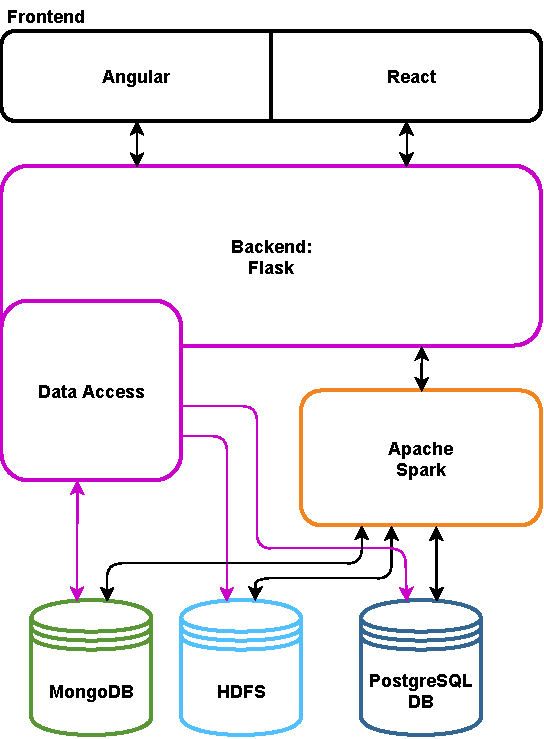
\includegraphics[scale=0.8]{graphics/data_lake_prototype_arch.pdf}}
\caption{Data Lake Prototype Architecture}
\label{DLPA}
\end{figure}

\subsection{Containerization}\label{CTN}
In recent years containerization is becoming more and more popular. 
The essencial function of a containerization-tool is that software can be installed and executed 
separtely from each other in an easy way. 

\textit{Docker} is a known and established containerization-tool, which we used in 
development and for testing.
Its advantages are that it can be used independent from the operating system as well as the 
number of computers one is using.
\textit{Docker} is also more lightweight than compareable solutions (e.g. virtual machines - VMs).
Containers are interchangeable, extendable and shippable to other computers.
\textit{Docker} enabled an error resistant development, because if a container did not work as 
intended anymore, the installations or changes simply could be undone.
The usage of \textit{Docker} also allowed us to execute the whole data lake on one computer with 
ease.

Important to notice is that using container for deployment is only a suggested approach.
Alternatives for implementing the data lake system are using VMs or installing the 
components of the data lake system on multiple servers.

%------------------------------------------------------------------------------------------------------
\section{Results}\label{RES}

\subsection{Ingestion Layer}\label{INL}

As described before, the ingestion layer is responsible for importing data from external 
heterogeneous sources in the data lake system. 
Therefore, the following information that is defined in the developed backend, has to be submitted 
to the ingestion layer.

\begin{table}[htbp]
\begin{center}
\begin{tabular}{|l|l|l|}
\cline{1-3} 
\textbf{\textit{argument}}& \textbf{\textit{required}}& \textbf{\textit{description}} \\
\hline
host & required & source host  \\
\hline
port & required & source port  \\
\hline
database & required & source database name \\
\hline
table or collection & required & source table- or collection-name\\
\hline
user & not required & source database user  \\
\hline
password & not required & source database password  \\
\hline
target storage system & not required & name of target storage system  \\
\hline
\end{tabular}
\label{TAB_DBI}
\end{center}
\caption{Arguments for Database Ingestion}
\end{table}

\begin{table}[htbp]
\begin{center}
\begin{tabular}{|l|l|l|}
\cline{1-3} 
\textbf{\textit{argument}}& \textbf{\textit{required}}& \textbf{\textit{description}} \\
\hline
file & required & source as file  \\
\hline
delimiter & not required & csv delimiter\\
\hline
hasHeader & not required & contains the first row a header\\
\hline
rowTag & not required & xml row tag\\
\hline
target storage system & not required & name of target storage system  \\
\hline
\end{tabular}
\label{TAB_FI}
\end{center}
\caption{Arguments for File Ingestion}
\end{table}

In detail, there are three different interfaces in the backend for the ingestion of raw data. 
One for the ingestion of collections from a \textit{MongoDB}, one for the ingestion of tables from a 
\textit{PostgreSQL} database and one interface for the ingestion of files, namely JSON, XML and CSV. 
If required, interfaces for different other source storage systems can be added with minor effort, 
because the overall construction of the ingestion layer and functions inside the developed backend 
are as generic and expandable as possible. 
Furthermore, it is uncomplicated to edit existing functionality to fit other required needs.

If the required information that were described before were submitted successfully, a new trackable 
job will be created in the backend. 
This job gets initialized with the start time and date of this job and also a short description of 
the work that needs to be done.
The user, who started the job will be saved as well.
After the job object was created and initialized successfully, its information is written in the 
database.
Afterwards the submitted data will be handed over to a newly created thread, to start the process of 
the ingestion. 
As the last step in this process, the ID of the job will be returned.
With this ID it is possible to track the process of the ingestion. 
The threading is a simple approach with an efficient result since no long-time requests are 
aborted by the client, because the server has not answered yet.

Figure~\ref{DBI} and figure~\ref{FI} show the communication between the variety of used 
components as well as the overall process of the ingestion. 
\textit{MongoDB} and \textit{PostgreSQL} ingestion are combined in Fig.~\ref{DBI}, because the procedure is quite 
similar for collections and tables.

In all three cases of the ingestion, the connection to the \textit{Spark}-cluster will be initiated
as the first step via a \textit{Spark}-session. 
If the connection is successfully established a DataFrame can be instantiated. 
This differs for the ingestion of a file, where a special step beforehand is required, as shown in 
Fig.~\ref{FI}.
Because \textit{Spark} cannot read in the submitted file directly from the developed backend, it 
needs to be written into a temporary folder inside the \textit{HDFS} of the used \textit{Hadoop}-cluster. 
To fulfill this requirement the \textit{Python} package \textit{WebHDFS} is used.
Another considered approach was, to copy the file to each existing node of the 
\textit{Spark}-cluster, so that \textit{Spark} can access the file on each node. 
This approach was too inefficient, so it was not used in the final prototype.

With the fully instantiated DataFrame it is possible to extract the schema of the source data. 
The extracted schema gets written in a metadata entry and gets stored, so it can be used for some 
use-cases, e.g. to annotate the fields embedded in the schema. 
After the extraction of the schema, it is stored in a local variable and the source data is 
written back to the given target storage system inside the data lake system. 
In this version of the data lake system no data quality requirements have been defined. 
The reason for this is the more general, prototype-like built of our data lake system. 
If data quality management is needed in a later version, where the overall purpose is specified
more precisely, it can be added. 
Every function in this layer was built with a possible data quality management in mind. 

The overall last step in the ingestion process is the creation of a metadata entry and the status 
update, of the earlier mentioned job that it succeded. 
The generated metadata entry will contain the user that started the ingestion, the time and date of
the ingestion, the extracted schema as well as source- and target-storage information. 
A detailed view of the used metadata model is shown in Fig.~\ref{MM} in the next section, the 
storage layer.

\begin{figure}[h]
\centerline{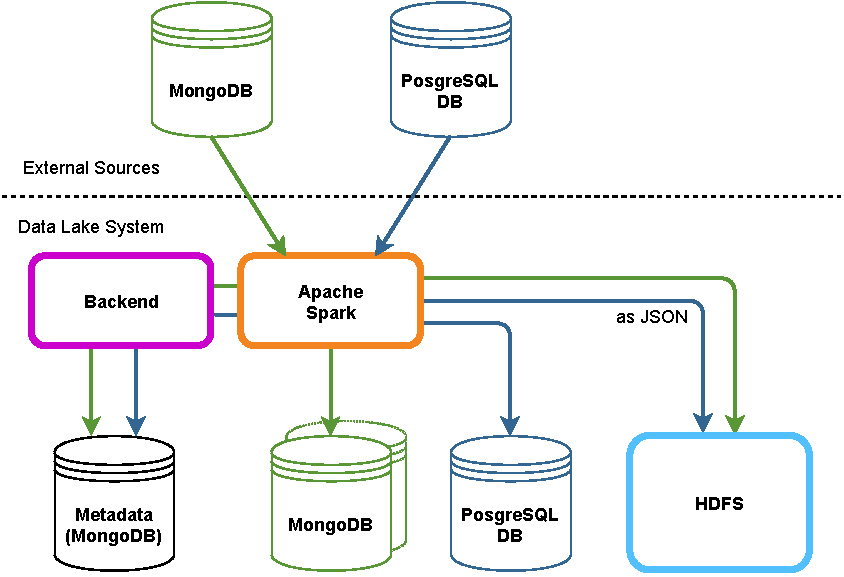
\includegraphics[scale=0.65]{graphics/db_ingestion.pdf}}
\caption{Data Base Ingestion}
\label{DBI}
\end{figure}

\begin{figure}[h]
\centerline{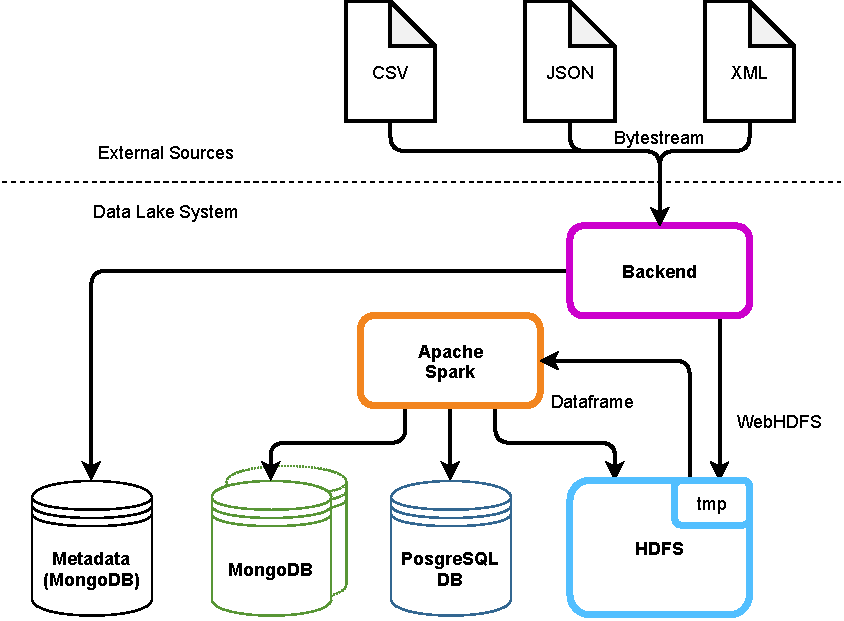
\includegraphics[scale=0.65]{graphics/file_ingestion.pdf}}
\caption{File Ingestion}
\label{FI}
\end{figure}

\subsection{Storage Layer}\label{STL}
There are various different database systems in the developed data lake to ensure the raw data
that was obtained during the ingestion can be stored in its source format and in a database system,
which is the same or at least a similar to the source database system. 
Any additional data obtained while working with the data lake, can also be stored in these storage 
systems. 

The metadata entries, mentioned already in the previous section, are stored in a \textit{MongoDB} and are 
accessed and managed with \textit{mongoengine}, an Object Document Mapper (ODM) for \textit{Python}. 
Besides the metadata entries, the user and job entries are also accessed and managed with 
\textit{mongoengine}. 
The use of \textit{mongoengine} greatly simplified the overall process of working with the metadata, which 
will be changed while working with the data lake. 
An example is the curating of the entries, where a user is annotating the extracted schema. 
A further advantage of \textit{mongoengine} is the variety of different, already integrated, functions like 
the efficient paging and searching. 
The overall reason for storing the metadata entries in a document-orienteted database like \textit{MongoDB}
are on the one side the flexibility and on the other side the scalability of \textit{MongoDB} instances. 
In that way, possible problems that may occur later on, could be bypassed because the defined model
is generic enough. 
In Fig.~\ref{MM} the used metadata model is shown in detail.

\begin{figure}[h]
\centerline{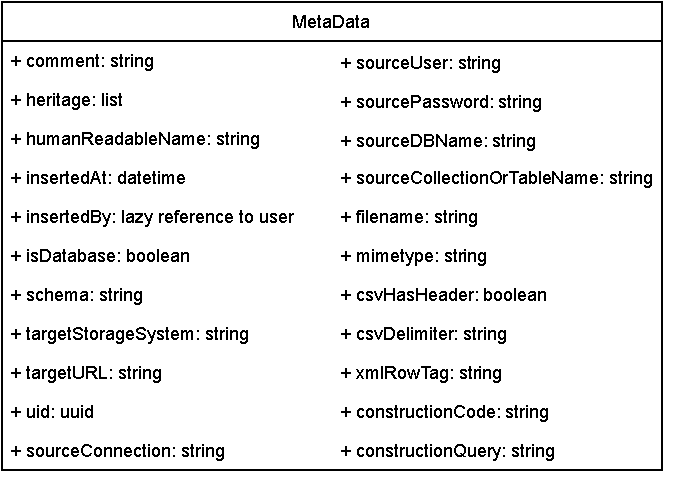
\includegraphics[scale=0.75]{graphics/metadata_model.pdf}}
\caption{Metadata Model}
\label{MM}
\end{figure}

As seen in the figure, the metadata entries were defined with the aim, to have a manageable 
complexity, so that the metadata entries can be exploited easily and understood by all variety of
users. 
To query the metadata entries later on, an additional index was created where each important 
metadata field was added. 
A scoring or weighting was not predefined, so that all fields are valued equally. 
If a different weighting is required, it can be added effortless to the metadata model.

As already mentioned before, the user has the possibility to choose the target storage system. 
If no target system is given, the following default mapping is used:

\begin{itemize}
\item[] Files $\to$ \textit{HDFS}
\item[] Tables $\to$ \textit{PostgreSQL}
\item[] JSON-Collections $\to$ \textit{MongoDB}
\end{itemize}

Otherwise, if a different target storage system is chosen, there will be a check, to ensure source 
and target storage system are compatible and there is no possible risk of data loss. 
Writing a CSV-, JSON- or XML-file to \textit{MongoDB} would make perfectly sense and will work. 
If one chooses to write a file to \textit{PostgreSQL}, this process will be prevented in our version of the
data lake.
When writing a collection in a \textit{PostgreSQL} database, it shall work in general but might not work 
properly in all cases. 
The reason for this is the possible data loss that results out of flattening the nested data. 

Overall, in most cases the better solution would be, to use the defined functions in the
transformation layer, to transform the source data to fit any target storage system. 
In all cases it is possible to bypass occurring problems of data loss or general 
incompatibility problems between source and target storage system. 

\subsection{Transformation Layer}\label{TFL}
In the transformation layer any data from the data lake storage can be loaded in \textit{Spark} and 
then be transformed into a different schema.
For transformation, \textit{PySpark} code and/or \textit{Spark SQL} queries can be executed on the 
loaded data.
The result of this transformation may then be stored in the data lake system as a so-called data 
mart.

To begin with, the name of the \textit{Spark}-session is received by the transformation layer, as 
well as a list of one ore more metadata entries.
If the \textit{Spark}-session does not already exist, a new one will be created.
There are several reasons for this that will be explained in the following.

\textit{Spark} provides temporary views in a local or global scope, which can be used to store data
without using DataFrames.
To prevent naming conflicts between views of different workflows, we chose to use local 
temporary views within a \textit{Spark}-session for each.
These views are used to store the result after each transformation, so it does not have to be 
recalculated on saving.

Next the process of a single transformation steps is explained in detail.
First, for every metadata entry and its identifier the source data get loaded in a DataFrame with 
the identifier as the variable name.
When all DataFrames are loaded, the provided \textit{PySpark} code, which was passed as a \textit{Python} 
script to the transformation layer, can be executed.
The \textit{Python} script is passed as a string and executed during runtime with the \textit{Python} function 
``exec".
If the execution was successfull all DataFrames are stored as a local temporary view to be available
to \textit{Spark SQL}. Then the given \textit{Spark SQL} queries can be executed on one or more of
these views.

In the later described dashboard, the transformation process differs in some aspects.
On the dashboard it is only possible to perform simple \textit{Spark SQL} queries on a single 
DataFrame. 
Therefore, the data should be transformed before they get loaded into the dashboard.

To greatly simplify the process of transforming the data, we built this layer in a way that made it 
possible to get intermediate results and have a more incremental work process.
In addition, these interfaces were defined with the goal to be able to integrate machine
learning algorithms at a later point of time. 

All gained results from all these described data interactions in this section can be written back 
into the data lake system.
Therefore, a target storage system has to be chosen to store the newly gained data. 
Before the data is written in the target storage system a metadata entry is generated with 
additional information like the heritage, construction code and construction query.
The new schema is extracted and saved as well. 

Referring to the heritage, this field was defined in the model to make each transformation and 
change trackable. 
This will help to understand, which processes were needed to transform the data, as viewed. 

\subsection{Interaction Layer}\label{IAL}
The interaction layer utilizes every other layer of the data lake to serve a single interface to 
clients for interacting with the data lake. 
The primary focus for this is set to the creation, reading, and transformation of the data, but it 
also should provide all neccessary functionalities to manage metadata and the ``user accounts"
respectively the authentication system.

The API was designed to be used independently from the client application and to be accessed
remotely.
For this purpose a REST API is an optimal solution. 
With this approach every client can connect to the server and use it as a backend. 
This backend can either be published over the internet to be publicly accessible or served in a 
private network.

The endpoints of the API must allow:
\begin{itemize}
    \item the starting of a new ingestion,
    \item reading and combining data from the data lake,
    \item access to the metadata for searching and managing and
    \item a simple authentication.
\end{itemize}
In the following these endpoints are described in detail.

The endpoint for starting an ingestion takes connection information of a datasource or the source
files itselfs and triggers the ingestion process. 
Next to the parameters that are required by the ingestion layer it also takes a ``human readable name" 
and a comment which both will be stored in the metadata.
For the implementation all default values for parameters that are optional on the 
REST API, but are required by the ingestion layer must be set first.
An example is the target storage system which is the source storage system by default. 
Then the ingestion is started and perceived by the client.

For reading data it is sufficient to load data from the storage layer and return it. 
To select the data that shall be read, the client has to pass the metadata ID so the interaction
layer can load the matching entry and extract the connection information. 
These information gets passed to the storage layer which returns the DataFrame holding the data.
The actual data and the schema are taken from this DataFrame.

The combination endpoint takes a selection of metadata IDs, identifier for each metadata, some 
\textit{PySpark} code, \textit{Spark SQL} code and a \textit{Spark}-session name. 
All of this information gets sent to the transformation layer which will return a preview of 
the result. 
This preview is a DataFrame of which data and schema will be returned to the client. 
A second option is to send a \textit{Spark}-session name for storing the result of the last 
transformation in the data lake. 
Therefore this endpoint is taking all neccessary parameters to write data.

The deleting of metadata takes an ID and deletes the entry and the corresponding data from the data
lake.

Managing metadata are simple create, read, update and delete operations on the metadata. 
In this case the comment, human readable name and the annotaions in the schema of a metadata entry 
can be edited.

For selecting the right metadata IDs for other endpoints there has to be a way to search for them.
This search takes a search string and returns a list of metadata entries which contain it.

A authentication enpoint assures that only permitted users can access the system.

In addition to the REST API the interaction layer contains a graphical user interface (GUI) to 
interact with.
For this implementation there are two different GUIs a user can use.
Both are web applications.

The first one is a dashboard which is provided by the \textit{Plotly} framework. 
The \textit{Plotly} framework makes it possible to create graphs and charts from a selected 
DataFrame. 
At the top the data of the DataFrame are shown in a table with optional filtering and paginagion. 
The dashboard has an input field to execute simple transformations on this DataFrame with 
\textit{Spark SQL} and another input field to enter \textit{Python} code, with which \textit{Plotly}
 figures can be generated.
It also allows to save the modified DataFrame in the data lake.

All of the remaining functionalities are implemented in a custom web application built with 
\textit{Angular}.
The \textit{Angular} client is devided into four different pages.
The first one shows a list of all jobs including their status and other information. 
It also contains a user interface to start a new ingestion.
Therefore the UI provides forms to enter all neccessary parameters to upload data. 
To always show the latest information on the jobs, primarily the current status of the job, the 
client periodically polls the backend.

A second view shows a table with a summary of the information about the metadata. 
Every row can be expanded to show the full information about source and target storage system, the 
schema and the heritage of this specific entry.
This view also allows editing of the metadata entries directly in the table.
Each entry has a button, which opens the corresponding dashboard in a new tab.
At the top is a search bar to look for specific metadata.

In another view the user is presented with multiple forms representing the workflow on the data. 
The first part is a search where the user can look for and select the required data.
For each selected entry an identifier must be set. 
These are the names, that are used as the variable names for the DataFrames in the \textit{PySpark}
code and as view names for \textit{Spark SQL}.
After the selection area, there are two input fields. 
The first, to enter the \textit{PySpark} code and the second can contain a \textit{Spark SQL} query. 
With the ``preview" button the user can access the combination endpoint, mentioned earlier, to 
generate a preview, which is shown in a table below. 
The amount of shown rows in the preview can be modified. 
If the preview matches the expected result the view contains a form at the bottom, where the user 
can enter the required information to store the result in the data lake.

The last view consists of a table with all registered users and a form to create or modify users.

%------------------------------------------------------------------------------------------------------
\section{Conclusion}\label{CON}
To summarize everything, the resulted data lake system is robust and widely useable as a base for
building more feature rich or specialized data lake systems in different contexts. 
Also its design allows to interchange most of the used frameworks with others.
The whole solution is currently designed and built to be used by experts. 

%------------------------------------------------------------------------------------------------------
\section{Outlook}\label{OUT}
To begin with, there are plenty of possibilities to extend the functionality of the data lake
system. 
The first and most obvious is the integration of other data source systems as needed.
Additional data quality management can be implemented to ensure the data in the system meets a 
specific standard. 

In the current state the ingestion of each data source is only done once. 
Continuous updating of the data marts is conceivable by either periodic fetching or with a 
implementation of a trigger system, so the data lake will get notified, if source data change. 
An important point will be the recalculation of every combined data mart with the new source. 
This is going to be a challenging task, especially when the system resources are limited. 

For extending the evaluation of data, machine learning processes are an usefull extension. 
``Machine learning can [be used for combining data from different] data silo[s] to 
optimize the operational business processes within an organization''\cite{Wibowo2017}, for example.
Because \textit{Spark} is used in this project, the implementation of machine learing in the data 
lake should be quite simple. 

At last the UI is a big field for further development and customization. 
Two possible ways are to either create an interface which can be used by everyone and not
only by experts, the second is to build a stripped down version for a specific use case.

%------------------------------------------------------------------------------------------------------
\begin{thebibliography}{00}
\bibitem{Quix2018} C. Quix and R. Hai, ``Data Lake''. In: \textit{Encyclopedia of Big Data Technologies}. Ed. by S. Sakr and
A. Zomaya. Cham: Springer International Publishing, 2018, pp. 1–8.
\bibitem{Dixon2010} J. Dixon. ``Pentaho, Hadoop, and data lakes''. In: \textit{blog, Oct} (2010).
\bibitem{Quix_Architecture} M. Jarke and C. Quix. ``On warehouses, lakes, and spaces – the changing role of conceptual
modeling for data integration.''. In: \textit{Conceptual Modeling Perspectives} (2017), pp. 231–245.
\bibitem{Wibowo2017} M. Wibowo, S. Sulaiman, and S. M. Shamsuddin. ``Machine Learning in Data Lake 
for Combining Data Silos''. In: \textit{Data Mining and Big Data}. Ed. by Y. Tan, H. Takagi, and 
Y. Shi. Cham: Springer International Publishing, 2017, pp. 294–306.
\end{thebibliography}

\end{document}
